%---------------------------------------------------------------------------%
\lecture{Research Presentation}{lec_present_intro}
%---------------------------------------------------------------------------%
\section{\enorcn{Model Setup}{引言}}%
%---------------------------------------------------------------------------%

% \begin{frame}[fragile]
%     \frametitle{Boussinesq Convection}
%     \vfill
%     % % \tikzart[t=m]{}% draw coordinate system
%     % \tikzart[t=p,x=-6.3,y=-1.5,w=4]{earth-science-volcanoes-339345-1280x1024}{\fullcite{test}}% position picture
%     % \tikzart[t=p,x=0,y=-1.5,w=4.2]{falk}% position picture
%     % \tikzart[t=p,x=5,y=-1.5,w=4]{moto_fins}% position picture
%     \begin{columns}
%         \begin{column}{.30\textwidth}
%             \centering
%             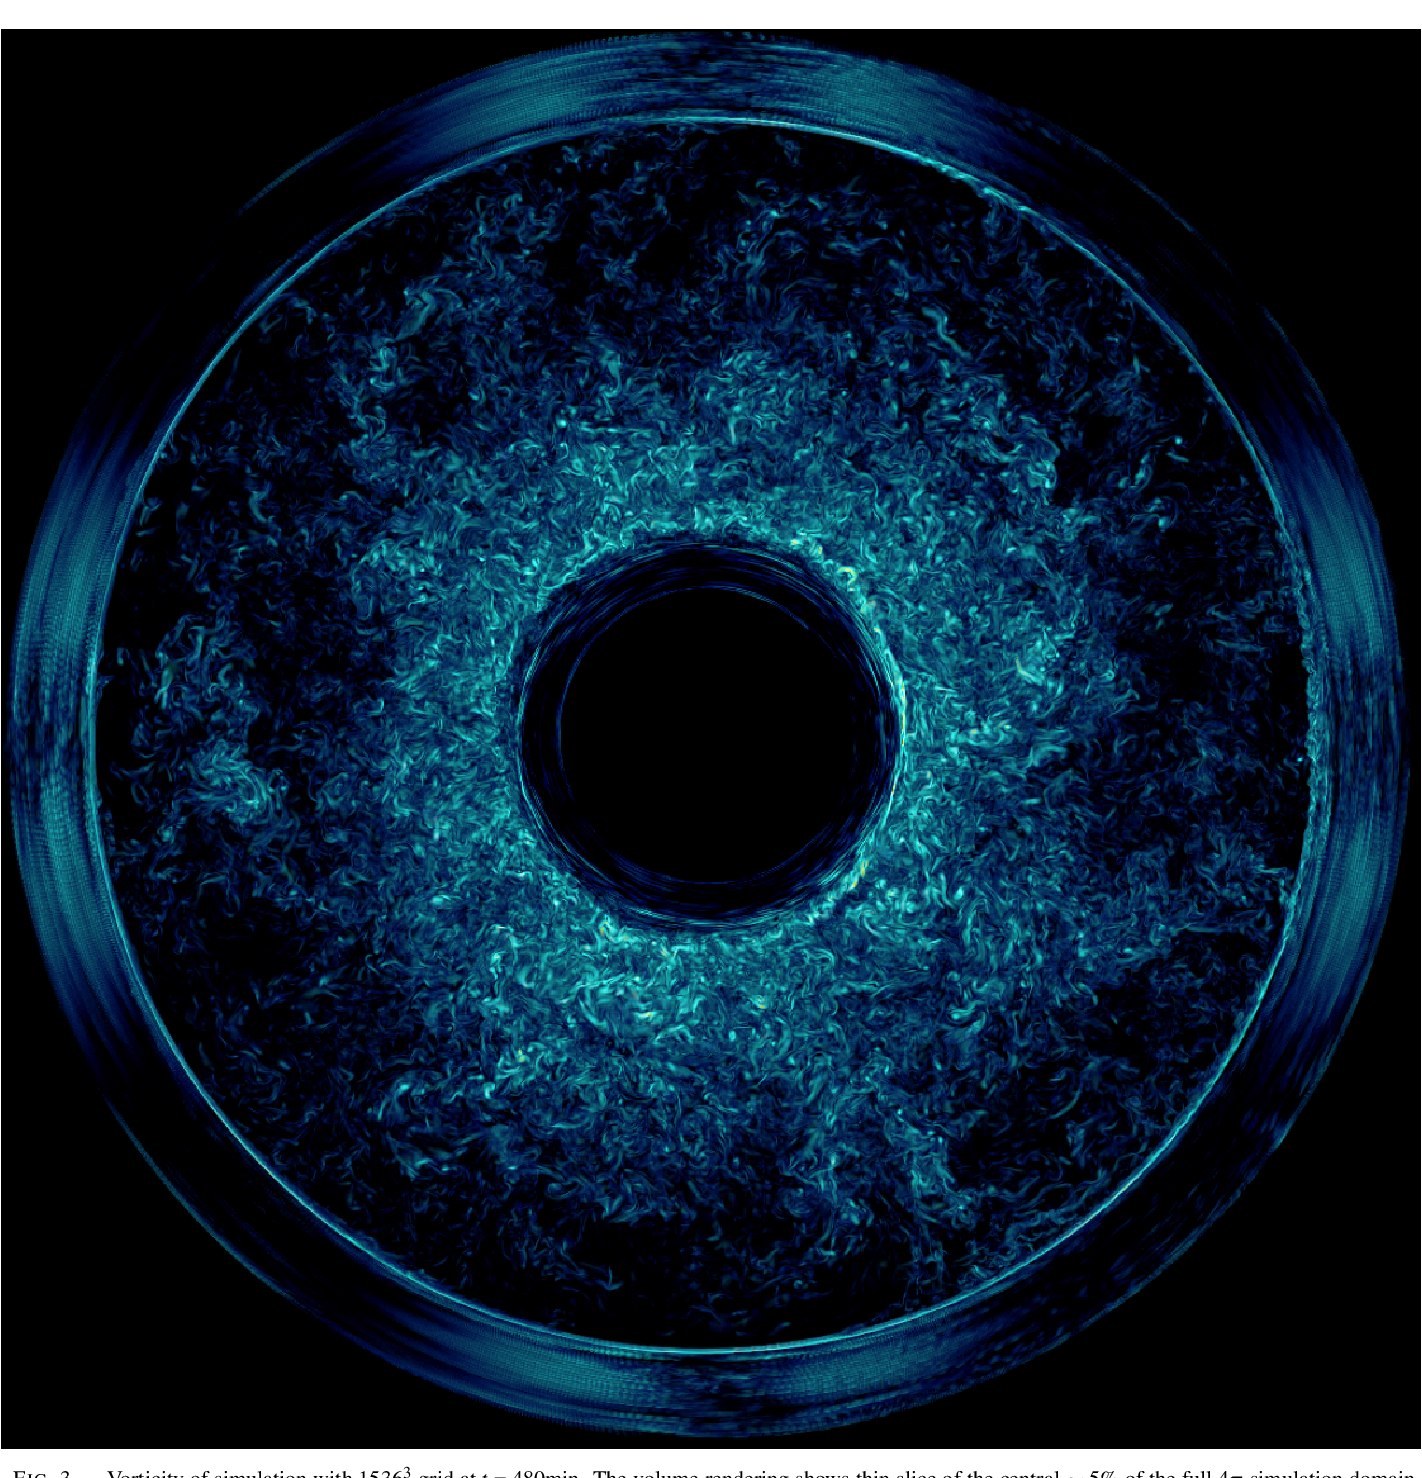
\includegraphics[height=0.8\textwidth]{falk.png}

%             {Astrophysics}
%         \end{column}

%         \begin{column}{.3\textwidth}
%             \centering
%             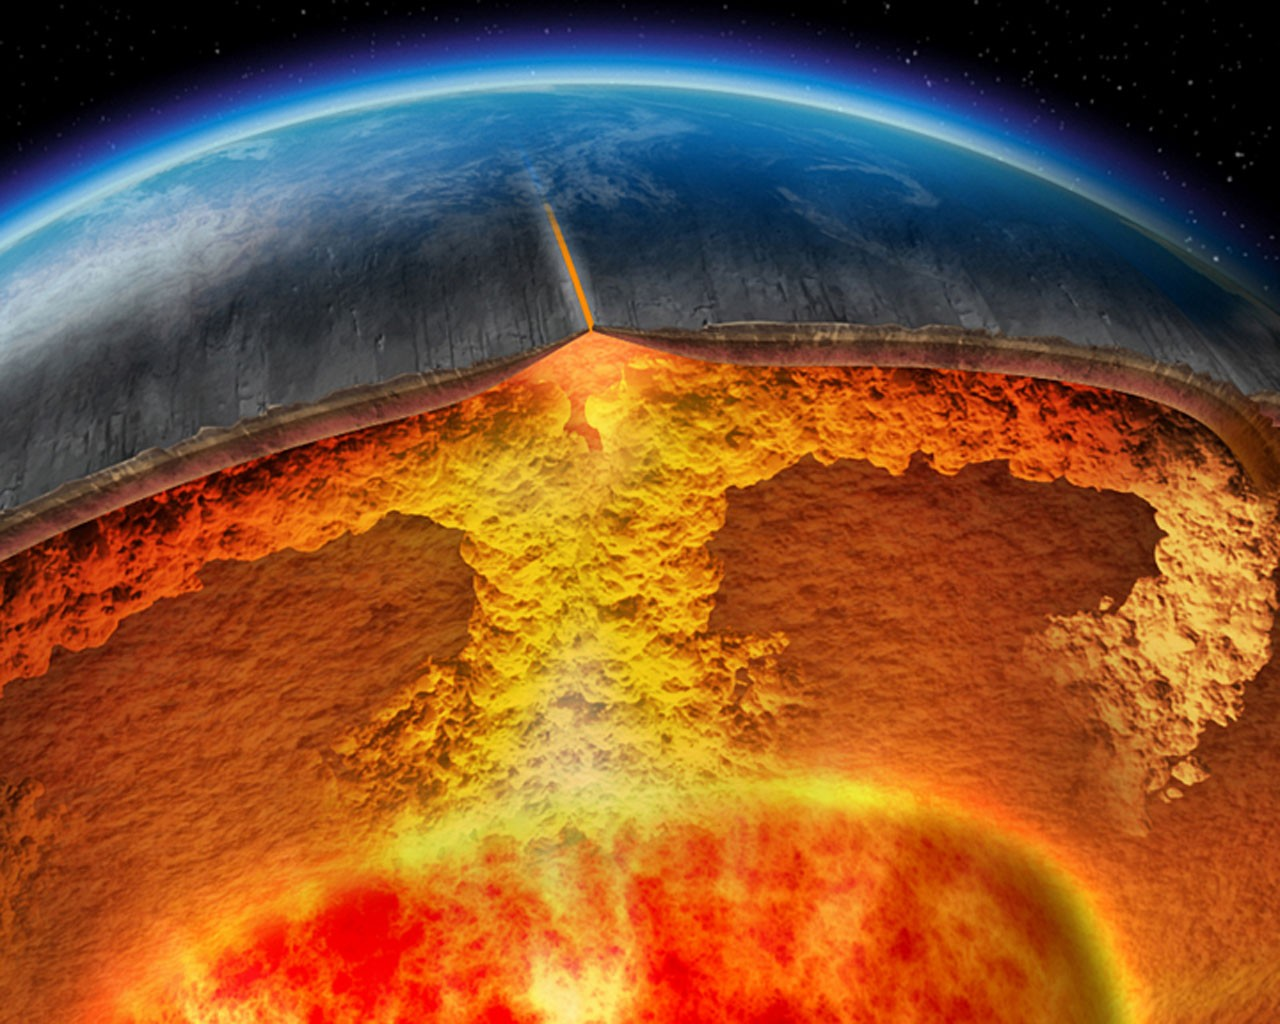
\includegraphics[height=0.8\textwidth]{earth-science-volcanoes-339345-1280x1024}

%             {Geophysics}
%         \end{column}

%         \begin{column}{.30\textwidth}
%             \centering
%             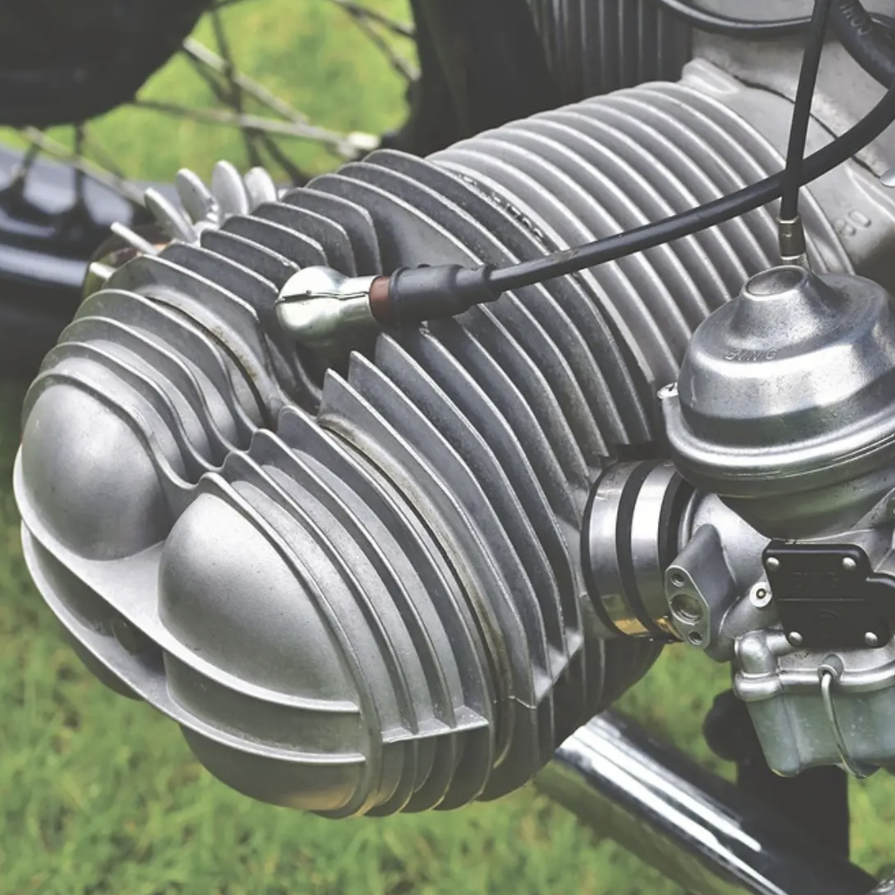
\includegraphics[height=0.8\textwidth]{moto_fins.png}

%             {Engineering}
%         \end{column}
%     \end{columns}
% \end{frame}

% \begin{frame}[fragile]
%     \frametitle{Why are we Still Studying Convection? \textbf{It's Elusive}}
%     \vfill
%     \begin{columns}
%         \begin{column}{.30\textwidth}
%             \centering
%             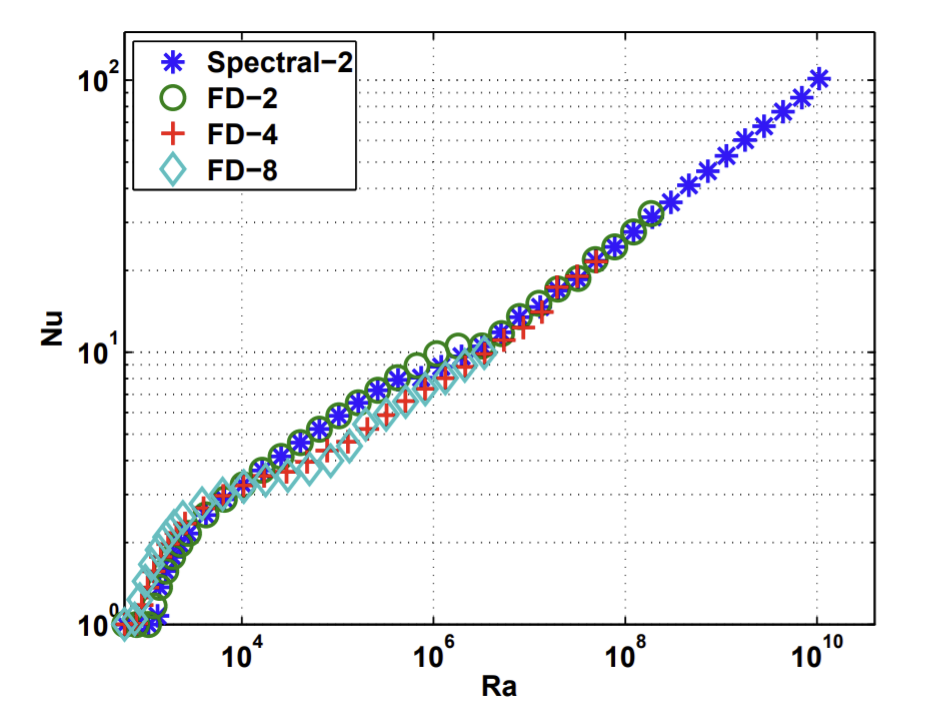
\includegraphics[height=0.85\textwidth]{johnson.png}

%             {(Johnson and Doering 2009)}
%         \end{column}

%         \begin{column}{.60\textwidth}
%             \centering
%             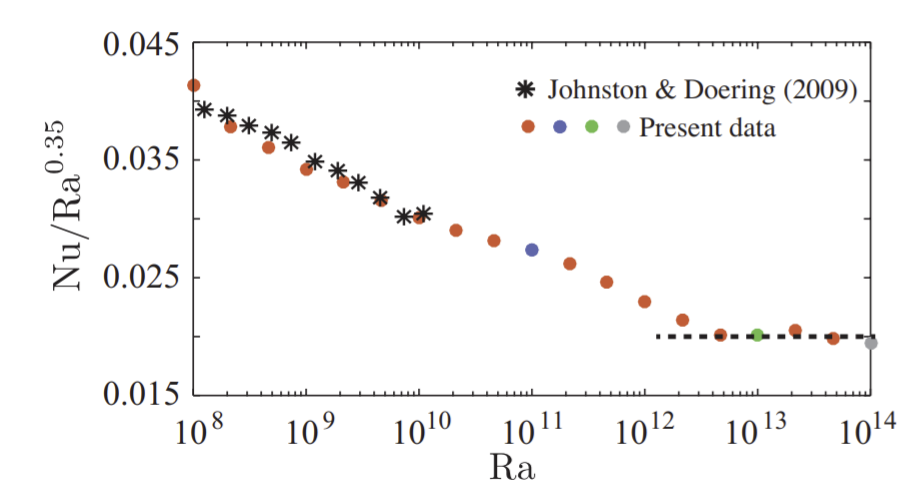
\includegraphics[height=0.5\textwidth]{zho.png}

%             {(Zhu et al 2019)}
%         \end{column}
%     \end{columns}
% \end{frame}

\begin{frame}[fragile]
    \frametitle{Boussinesq Convection: The PDE}
    \begin{itemize}
        \item Incompressible kinematics with buoyancy term
        \begin{align}
            \nabla \cdot \vec{u} &= 0 \label{EQ:motion1}\\
            \frac{\partial \vec{u}}{\partial t} + \vec{u} \cdot \nabla \vec{u} &= - \nabla p + T \hat{z} + \mathcal{R} \nabla^2 \vec{u} \label{EQ:motion2}\\
            \frac{\partial T}{\partial t} + \vec{u} \cdot \nabla T &= \mathcal{P} \nabla^2 T \label{EQ:motion3}
        \end{align}
        where $\vec{u},T,$ and $p$ and velocity, temperature, and pressure respectively.
        \vspace{0.2cm}
        \item Momentum diffusivity: $\mathcal{R} = \sqrt{\frac{\Pr}{\Ra}}$ 
        
        \item Thermal diffusivity: $\mathcal{P} = \frac{1}{\sqrt{\Pr \Ra}}$.
    \end{itemize}
\end{frame}


\begin{frame}[fragile]
    \frametitle{Boussinesq Convection: Miscellaneous Prescriptions}

    \begin{itemize}
        
        \item Nondimensionalized on the freefall timescale\newline
        \item Domain: $\mathcal{D}=\{ (x,z)\;|\; x\in(0,4),\; z\in(-1/2,1/2)\}$\newline
        \item Prescribed-temperature:
        $T|_{z=-1/2}(x,t)=1/2, \; T_{z=1/2}(x,t)=-1/2$\newline

        and no-slip impenetrable $\vec{u}|_{z=\pm1/2}(x,t) = \vec{0}$ boundary conditions\newline

        \item Fixed Prandtl number $\rm{Pr}=1$, varied Rayleigh number $10^6\leq \rm{Ra}\leq 10^9$
    \end{itemize}
\end{frame}

%---------------------------------------------------------------------------%

%---------------------------------------------------------------------------%
